\documentclass[10pt, a4paper]{article}

% On écrit en français
\usepackage[utf8]{inputenc}
\usepackage[frenchb]{babel}
\usepackage[T1]{fontenc}

% Packages nécessaires
\usepackage{graphicx}
\usepackage{hyperref}

% Numérotation de page custom
\usepackage{fancyhdr}
\usepackage{lastpage}
\pagestyle{fancy}
\fancyhf{}
\rfoot{Page \thepage \hspace{1pt} sur \pageref{LastPage}}

% Police Helvetica <3
\usepackage{helvet}
\renewcommand*{\familydefault}{\sfdefault}

% Enlever les alinéas
\setlength{\parindent}{0pt}

% Marges plus larges pour faire moins LaTeX
\usepackage[left=3cm, right=3cm]{geometry}

% Sous titre de document
\usepackage{titling}
\newcommand{\subtitle}[1]{%
  \posttitle{%
    \par\end{center}
    \begin{center}\large#1\end{center}
    \vskip0.5em}%
}

% En tête complet de document
\newcommand{\Document}[1]{%
    \title{#1}
    \subtitle{Dématérialisation d'un processus de paiement}
    \author{
        COMETS Jean-Marie \\
        DELMARRE Adrian \\
        REYNOLDS Nicolas \\
        TURPIN Pierre
    }
    \date{\today}

    \maketitle \newpage

    \tableofcontents \newpage
}


\begin{document}

\Document{Architecture technique}

\section{Présentation générale}

Dans la suite du document, les sous-systèmes suivront la nomenclature suivante:

\begin{description}
    \item[serveurs de dialogue borne] la machine contenant le serveur de
        dialogue principal sera noté $B$, les machines de repli seront notées
        $Bn$.
    \item[serveurs de base de données] la machine contenant le serveur de base
        de données principal (maître) sera noté $BDD$, les duplicats seront
        notés $BDDn$, les archives seront notées $BDDa$.
    \item[serveurs d'application] la machine contenant le serveur d'application
        principal sera noté $X$, les machines de repli $Xx$, avec $X$
        respectivement $E$, $C$, $U$ et $A$ pour les applications "gestion
        commerçant", "gestion entreprise", "gestion utilisateur" et "gestion
        Aventix".
    % TODO ajouter les nomenclatures manquantes
\end{description}

\section{Choix de la solution cloud}
\section{Passage à l'échelle (scaling)}

\section{Sécurité}

\subsection{Infrastructure}

En choisissant une solution cloud, la disponibilité de l'infrastructure est
garantie par le prestataire cloud, en l'occurence \textbf{Amazon AWS}. Le
système peut donc être considéré relativement sécurisé vis-à-vis des attaques
par déni de service (DoS simple), ou autre attaque d'infrastructure. \\

De plus, la disponibilité du système est dépendante de la disponibilité d'AWS,
en l'occurence celle-ci peut être garantie selon le prix de la prestation. Le
taux de panne de 0\% ne peut malheureusement pas être garanti, du fait du
nombre de facteurs externes entrant en jeu. Cependant, un taux de 99\%, voire
jusqu'à 99.95\% peut être garanti par AWS. \\

En passant par une solution cloud, le système est aussi protégé des attaques
physiques (coupure générale, attaque électromagnétique, etc...), mais encore
dépendant de l'infrastructure d'AWS.

\begin{figure}[h]
    \centering
    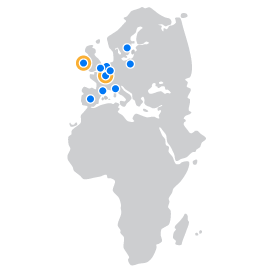
\includegraphics[width=0.7\textwidth]{aws-europe}
    \caption{Emplacements géographiques possibles des instances EC2}
    \label{fig:aws-europe}
\end{figure}

\subsection{Gestion du trafic indésirable}

Le trafic indésirable correspond au trafic qui n'est pas directement lié à
l'utilisation normale du système. Il peut être utilisé comme attaque visant à
réduire exploiter des failles d'autres services présents sur la VM, ou tout
simplement visant à réduire la disponibilité du système en multipliant les
accés (DoS). \\

EC2 met à disposition un firewall pour ses instances, ce qui permet de régler
son accés. Cependant, les VM étant installées à l'intérieur d'une instance,
elles doivent toutes être configurées séparément pour accepter uniquement le
trafic qui les concerne.

\subsubsection{Fermeture maximale}

Un document relatant des conseils de sécurisation d'instance EC2, produit par
ce même service, est disponible à l'adresse suivante :
\url{http://aws.amazon.com/articles/1233/} (en date du \today).

\end{document}
